\exercise{Part 1 - Link between online learning and game theory}

All the code is written in the Python script \texttt{homework.py}.

\question{1.} For the game "Rock Paper scissors", we define the actions rock $= 1$, paper $= 2$, scissors $= 3$. The loss matrix L is as follows 
\begin{equation*}
	L = \begin{pmatrix}
		0 & 1 & -1 \\
		-1 & 0 & 1 \\
		1 & -1 & 0
	\end{pmatrix}
\end{equation*}


\question{2. (a)} We implement the function $\mathtt{rand\_weighted(p)}$ that samples $\i \in [| M |]$ with respect to the distribution $p \in \Delta_M$. In Python, the function is simply
\begin{lstlisting}
def rand_weighted(p) :
	return np.argwhere(np.cumsum(p) > np.random.rand())[0, 0]
\end{lstlisting}
In this function, we build an array \texttt{c = np.cumsum(p)} that contains the cumulative probabilities of p i.e $c_i = p_1 + ... + p_i$. We then sample a number $x \in [0, 1)$ and determine the first index i in the 
cumulative array c such that $c_i > x$. It is easy to show that for all j, $i = j$ with probability $p_j$. 

\question{2. (b)} To implement the function \texttt{EWA\_update(p, l)} we simply multiply the vectors p and $\exp{(- \eta  l_t(i) )}$ component-wise and then normalize the new vector.

\question{3. (a.))}  We simulate EWA against a fixed adversary with strategy $q = (0.5, 0.25, 0.25)$, in the function \texttt{EWA(L, T, eta, q}. This function runs T iterations. At iteration t, we sample an action $j_t$ from q using \texttt{rand\_weighted} and update the weights $p_t$ with the function \texttt{EWA\_update} called with the loss $l_t$. The loss $l_t(i)$ of the player if he choses the action $i$ is equal to $L(i, j_t)$. 

\question{3. (b)} As asked, we simulate the game with $T = 100, \eta = 1.0$ and plot the weight vectors $p_1, ..., p_T$ in the figure (\ref{fig:question3b}) . We see that the best strategy is $p = (0.0, 1.0, 0.0)$. We can prove it rigorously. Indeed, consider the strategy $p =(x, y, z)$ that minimizes the average loss $l(p, q) = \mathbb{E}_{i \sim p, j \sim q}(L(i, j))$. We write 
\begin{align*}
	l(p, q) &= x \times (0.25 - 0.25) + y \times (0.25 - 0.5) + z \times (0.5 - 0.25) \\
	&= -0.25 \times y + 0.25 \times z
\end{align*}
The optimal value of p that satisifies the constraint $p \in \Delta_3$ and minimizes the above expression is $x = 0, y = 1, z = 0$ which is what we wanted. 

\begin{figure}
	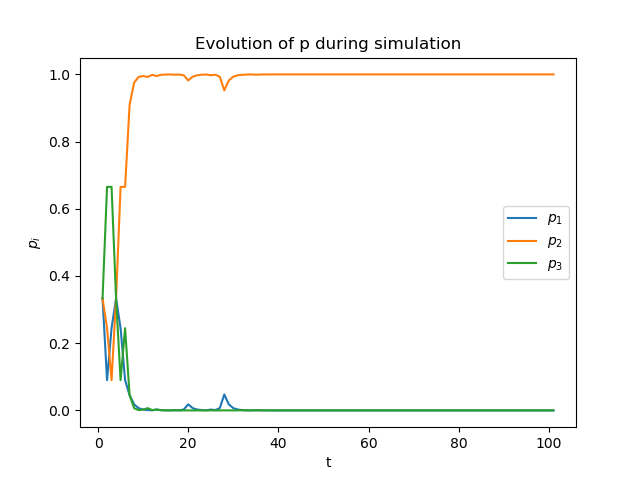
\includegraphics[width=\textwidth]{images/question3b}
	\caption{Plot of the player's stragegy p with \texttt{EWA}, when opponent has a fixed strategy (0.5, 0.25, 0.25)}
	\label{fig:question3b}
\end{figure}

\question{3. (c)} We plot the average loss $\bar{l}_t = \frac{1}{t} \sum_{1 \leqslant s \leqslant t} l(i_s, j_s)$ as a function of t, and obtain the figure (\ref{fig:question3c}). The figure shows 10 different runs of the simulation.  

\begin{figure}
	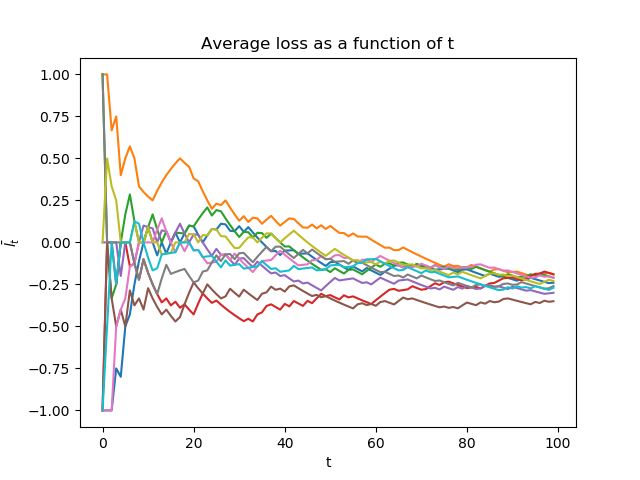
\includegraphics[width=\textwidth]{images/question3c}
	\caption{Plot of the average loss as a function of t for 10 simulations of the game with \texttt{EWA}}
	\label{fig:question3c}
\end{figure}

% TODO : question 3.(d) redaction
\question{3. (d)} Here, the cumulative regret is defined by 
\begin{equation}
	R_t = \sum_{s = 1}^t L(i_s, j_s) - \underset{i}{\min} \sum_{s \leqslant t}L(i, j_s)
\end{equation}. Figure (\ref{fig:fig:question3d})

\begin{figure}
	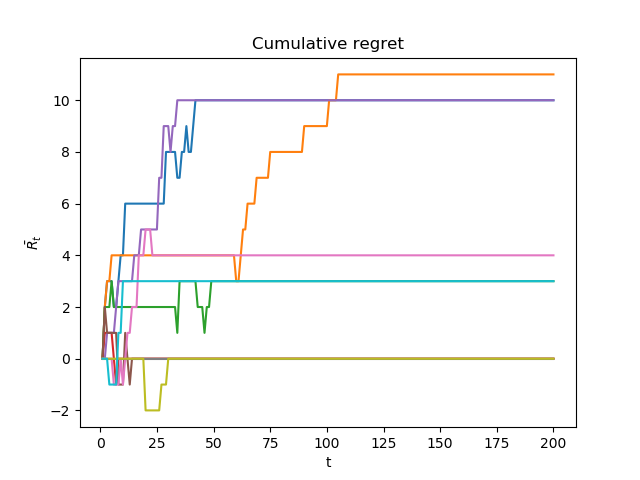
\includegraphics[width=\textwidth]{images/question3d}
	\caption{Cumulative regret $R_t$ for 10 simulations}
	\label{fig:question3d}
\end{figure}

% TODO : question 3(e) : justification theorique
\question{3. (e)} To estimate the stability, n = 10 simulations are executed, and we plot in figure (\ref{fig:question3e}) the n average losses as well as the minimum, maximum and mean losses. At first glance, the \texttt{EWA} seems to be stable. Indeed, the maximum and minimum both seem to converge towards the value $l_\infty = -0.25$.

\begin{figure}
	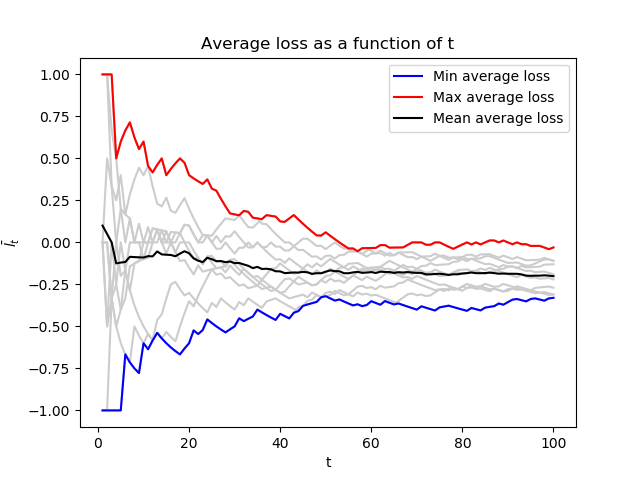
\includegraphics[width=\textwidth]{images/question3e}
	\caption{Average, minimum and maximum of the average loss $\bar{l}_t$. The n average losses are plotted in grey.}
	\label{fig:question3e}
\end{figure}

% TODO : question 3(f) comparaison des learning rates en pratique
\question{3. (f)}
In theory, the best learning rate $\eta$ with \texttt{EWA} is $\eta_{\text{EWA}} = \sqrt{2 ln(K) / T}$ with $K = 3$ here and $T = 100$, so we obtain $\eta_{\text{EWA}} \simeq 0.15$. We see that in practice, the best learning rate is not necessarily equal to $\eta_{\text{EWA}}$. 

\question{4. (a)} \textit{Simulation against an adaptive adversary}
When the adversary uses \texttt{EWA} like the player, we observe that the average loss seems to converge towards 0 which is the value of the game.

\begin{figure}
	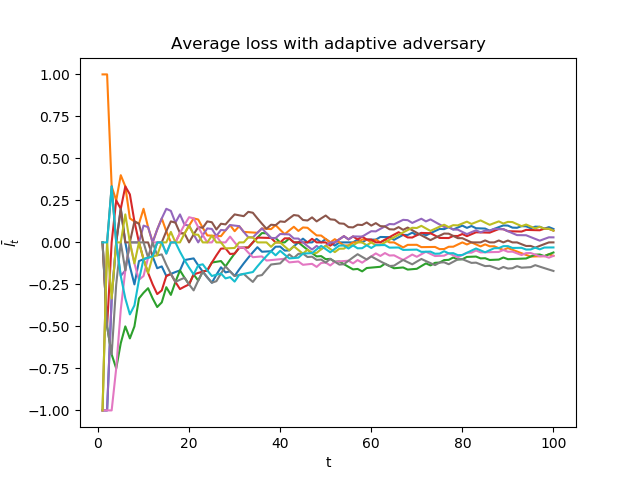
\includegraphics[width=\textwidth]{images/question4a}
	\caption{Average loss for n = 10 simulations with adaptive adversary}
	\label{fig:question4a}
\end{figure}

% TODO : question 4(b). Comprendre pourquoi la distance ne converge pas vraiment vers 0
\question{4. (b)}

\paragraph*{Bandit feedback} We now assume that the player doesn't have access to L but only the incured loss $L(i_t, j_t)$. We implement the algorithm \texttt{Exp3} where at each time t, the action $i_t$ is selected with a probability
$$
\mathbb{P}(i_t = i) = \frac{\exp{(- \eta \hat{l_t}(i))}}{\sum_j \exp{(- \eta \hat{l_t}(j))}}
$$
where $\hat{l_t}(i)$ is the \textit{estimated loss} of the action i, i.e the average loss incured by the player when the action i was selected. 